\begin{frame}{Clinical Artifact 3: Pulse Oximetry Bias}
\begin{center}
\IfFileExists{../analysis_artifacts/fig3_pulseox_bias.pdf}{\includegraphics[width=0.92\textwidth,height=0.66\textheight,keepaspectratio]{../analysis_artifacts/fig3_pulseox_bias.pdf}}{%
\IfFileExists{../analysis_artifacts/fig3_pulseox_bias.png}{\includegraphics[width=0.92\textwidth,height=0.66\textheight,keepaspectratio]{../analysis_artifacts/fig3_pulseox_bias.png}}{%
\IfFileExists{../analysis_artifacts/occult_hypoxemia.pdf}{\includegraphics[width=0.92\textwidth,height=0.66\textheight,keepaspectratio]{../analysis_artifacts/occult_hypoxemia.pdf}}{%
\begin{tikzpicture}
\begin{axis}[ybar,width=0.95\textwidth,height=0.58\textheight,ymin=0,ymax=32,ylabel={Occult hypoxemia rate (\%)},symbolic x coords={White,Hispanic,Asian,Black},xtick=data,bar width=6pt,legend style={at={(0.5,1.05)},anchor=south,legend columns=2,font=\scriptsize}]
\addplot coordinates {(White,3.6) (Hispanic,0) (Asian,0) (Black,11.7)};
\addplot coordinates {(White,17.2) (Hispanic,29.8) (Asian,30.2) (Black,28.5)};
\legend{Sjoding 2020 signal,Fawzy 2022 COVID cohort}
\end{axis}
\end{tikzpicture}}}}
\end{center}
\small The defensible diagnostic case is pulse oximetry, where missing calibration context caused unequal reliability during COVID care.
\end{frame}
